\documentclass[serif,professionalfont]{beamer}

\usepackage{code}

\usepackage{tikz}
\usetikzlibrary{shapes,arrows,calc}

\usepackage{amssymb}

\usepackage{hyperref}

\usepackage{mathpartir}
\usepackage{color}

% Helvetica
% \usepackage[scaled]{helvet}
% \renewcommand*\familydefault{\sfdefault} %% Only if the base font of the document is to be sans serif
% \usepackage[T1]{fontenc}

% Latin Modern Sans
\usepackage{lmodern}
\renewcommand*\familydefault{\sfdefault} %% Only if the base font of the document is to be sans serif
\usepackage[T1]{fontenc}

\usepackage{amsmath}
\usepackage{array}
\providecommand{\alert}[1]{\textbf{#1}}

% \definecolor{Purpleee}{RGB}{140,20,140}
% \definecolor{PurpleL}{RGB}{255,170,255}
% \definecolor{MyGreen}{RGB}{5,95,5}
% \setbeamercolor{title}{fg=Purpleee}
% \setbeamercolor{frametitle}{fg=Purpleee}
% \setbeamercolor{structure}{fg=Purpleee}


\usepackage{listings}

\lstnewenvironment{codex}[1][]%
  {
   \noindent
   \minipage{\linewidth}
   \vspace{0.2\baselineskip}
%   \vspace{-0.4\baselineskip}
   \lstset{basicstyle=\ttfamily,
%           frame=single,
           language=Haskell,
           keywordstyle=\color{black},
           #1}}
  {%\vspace{-0.8\baselineskip}
   \endminipage}

\title{ {\huge Static Haskell Contract Checking} }
\institute{ Microsoft Research }

\author{ {\Large Dan Ros\'en}
     \vspace{\baselineskip} \\
     Dimitrios Vytiniotis, Koen Claessen, Simon Peyton Jones}
\date{September 5, 2012}


\begin{document}

\maketitle
\makeatactive

\newcommand{\Th}[0]{{\cal T}}
\newcommand{\alttr}[1]{#1^{m}}
\newcommand{\ol}[1]{\overline{#1}}
\newcommand{\Ct}{{\tt C}}
\newcommand{\CF}{{\tt CF}}
\newcommand{\roll}[1]{#1}
\newcommand{\unroll}[1]{#1}
\newcommand{\bind}[2]{#1(#2)}
\newcommand{\ret}[1]{#1}
\newcommand{\injK}[2]{\mathsf{#1}(#2)}
\newcommand{\injKZ}[1]{\mathsf{#1}}
\newcommand{\injFun}[1]{\mathsf{Fun}(#1)}
\newcommand{\injBad}{\mathsf{Bad}}
\newcommand{\dbrace}[1]{[\![#1]\!]}
\newcommand{\Fcf}{F_{\lcfZ}}
\newcommand{\lcfZ}{\textsf{cf}}
\newcommand{\dapp}{\mathsf{app}}
\newcommand\cf[0]{\mathsf{CF}}
\newcommand\conj[0]{\&}
\newcommand\cons[2]{\mathsf{cons}(#1,#2)}
\newcommand\conspi[1]{\mathsf{cons_0}(#1)}
\newcommand\conspii[1]{\mathsf{cons_1}(#1)}
\newcommand\nil[0]{\mathsf{nil}}
\newcommand\head[1]{\mathsf{head}(#1)}
\newcommand\maps[0]{\mathsf{map}}
\newcommand\map[2]{\maps(#1,#2)}
\newcommand\ptr[1]{#1_\mathsf{ptr}}
\newcommand\app[2]{\mathsf{ap}(#1,#2)}
\newcommand\appp[3]{\app{\app{#1}{#2}}{#3}}
\newcommand\unr[0]{@UNR@}
\newcommand\True[0]{@True@}
\newcommand\False[0]{@False@}
\newcommand\bad[0]{@BAD@}
\newcommand\formula[1]{#1}
\newcommand\highlight[1]{#1}
\newcommand{\taus}{\ol{\tau}}
\newcommand{\interp}[3]{[\![#1]\!]} %_{\langle {#2},{#3}\rangle}}
\newcommand{\etrans}[3]{{\cal E}\{\!\!\{#3\}\!\!\}}
\newcommand{\ptrans}[2]{{\cal P}\{\!\!\{#2\}\!\!\}}
\newcommand{\trc}[1]{{\cal C}\{\!\!\{#1\}\!\!\}}
\newcommand\Min[0]{\mathsf{min}}


\begin{frame}[fragile]
  \frametitle{Contracts}

  Express correctness of Haskell programs with \emph{contracts}.

  \[\begin{array}{lcll}
    C & ::=  & (x : C) \to C  & \text{dependent function space} \\
      & \mid & \{ x \mid p \} & \text{predicates} \\
      & \mid & \cf            & \text{crash free} \\
      & \mid & C \conj C      & \text{conjunction} \\
  \end{array}\]

  Predicates declared with Haskell functions with ordinary semantics. Examples:

  \[\begin{array}{l}
    @head@ \in \cf \to \cf \\
    @head@ \in \{ @xs@ \mid @not (null xs)@ \} \to \cf \\
    @head@ \in \cf \conj \{ @xs@ \mid @not (null xs)@ \} \to \cf \\
    @filter@ \in (p : \cf \to \cf) \to \cf
                \to \cf \conj \{ ys \mid @all@ \; p \; ys \}
  \end{array}\]

\end{frame}

\begin{frame}[fragile]
  \frametitle{Motivation}

  \begin{itemize}

    \item Related work:
      Xu using wrapping, recent work for OCaml

    \item Interesting aspects of Haskell:
      \begin{itemize}
        \item lazy/infinite data structures,
        \item higher-order,
        \item pure
      \end{itemize}
  \end{itemize}

\end{frame}

\begin{frame}[fragile]
  \frametitle{Overview}

  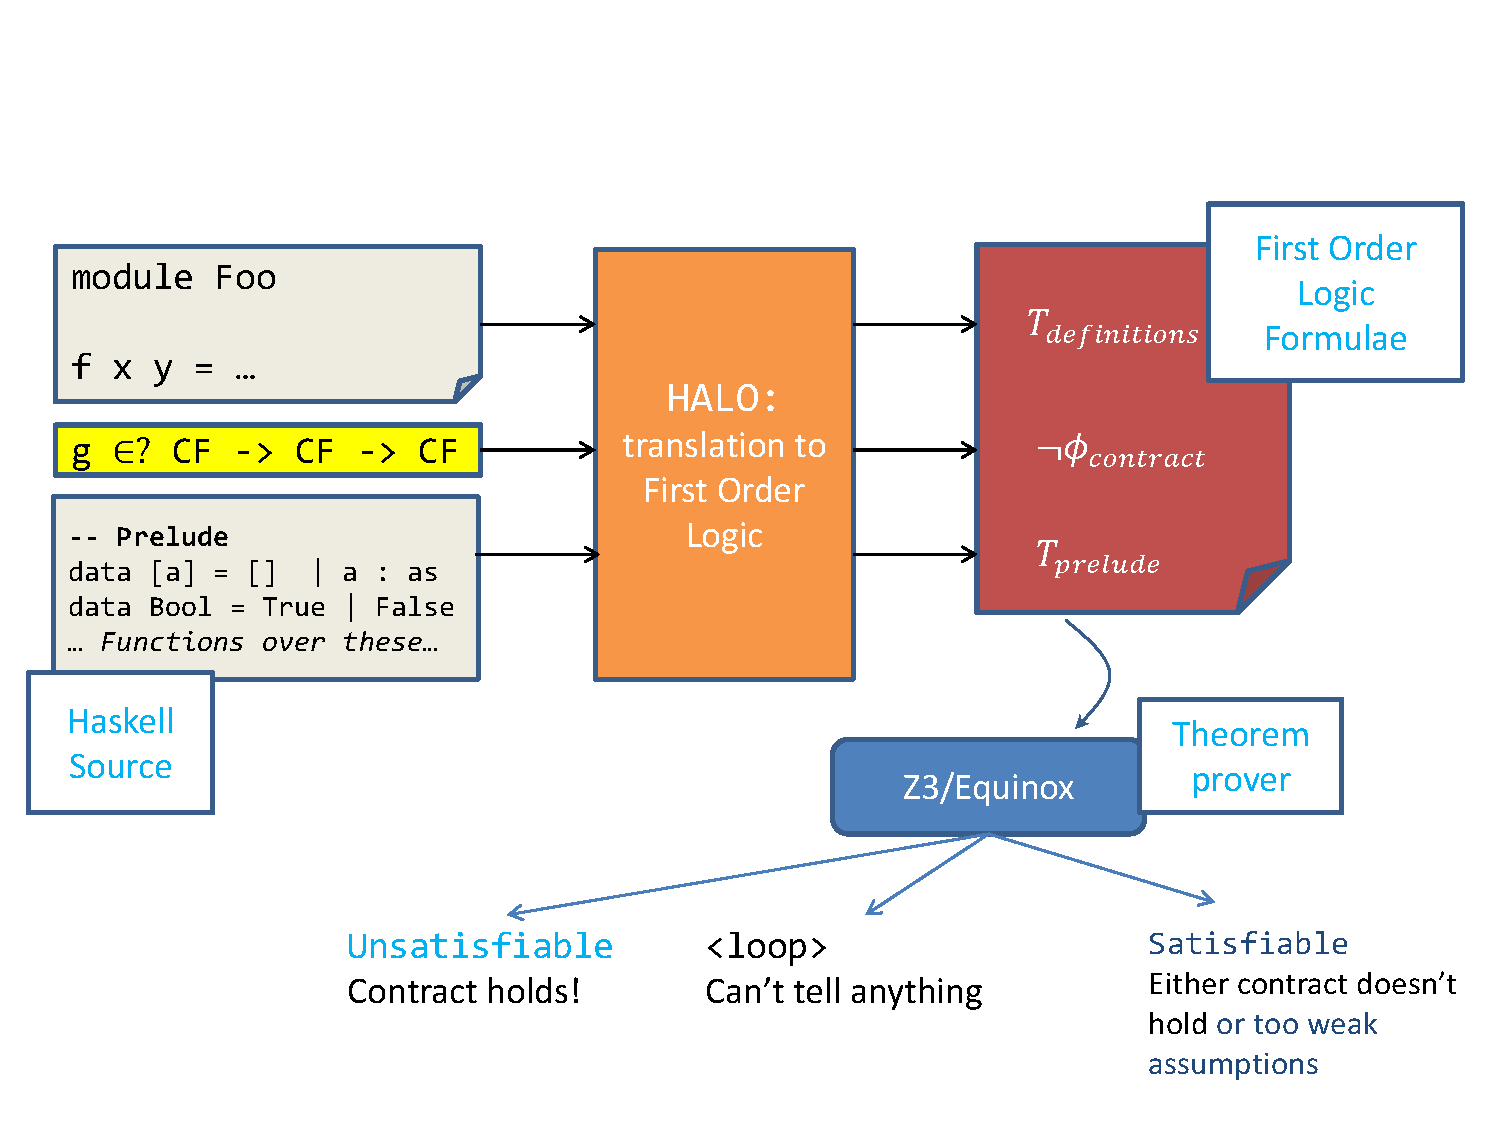
\includegraphics[width=\textwidth]{overview.pdf}

\end{frame}

\begin{frame}[fragile]
  \frametitle{Denotational semantics}

  Idea: translate a denotational model to FOL.

  \begin{itemize}
    \item Discrimination axioms

    $$
    \cons{x}{xs} \neq \nil \neq \unr \neq \bad
    $$

    \item Injectivity axioms

    \[\begin{array}{lcl}
      \conspi{\cons{x}{xs}} & = & x, \\
      \conspii{\cons{x}{xs}} & = & xs
    \end{array}\]

    Using $\mathsf{cons_0}$ we have $\cons{x}{xs} = \cons{y}{ys} \to x = y$.
  \end{itemize}

\end{frame}

\begin{frame}[fragile]
  \frametitle{Guiding principle for translation to FOL}

  \begin{theorem}
  Assume that $\Sigma \vdash P$ and $e_1$ and $e_2$ contain no free term variables. The following
  are true:
  \begin{itemize}
    \item $\dbrace{e_1} = \dbrace{e_2}$ iff ${\cal I}(\etrans{}{}{e_1}) = {\cal I}(\etrans{}{}{e_2})$.
    \item If $\Th \land \ptrans{\Sigma}{P} \vdash \etrans{}{}{e_1} = \etrans{}{}{e_2}$ then $\dbrace{e_1} = \dbrace{e_2}$.
  \end{itemize}
  \end{theorem}
  \[\begin{array}{cc}

    \begin{array}{rcl}
%    \multicolumn{3}{l}{\interp{e}{\cdot}{\cdot} : (\FVarCpo =>_c D_{\infty}) \times (\VarCpo =>_c D_{\infty}) =>_c D_{\infty}} \\
      \interp{x}{\sigma}{\rho}                    & {=} & \rho(x) \\
      \interp{f}{\sigma}{\rho}           & {=} & \sigma(f) \\
      \interp{K\;(\ol{e})}{\sigma}{\rho} & {=} & \roll{\ret{\injK{K}{\ol{\interp{e}{\sigma}{\rho}}}}} \\
      \interp{e_1\;e_2}{\sigma}{\rho}             & {=} & \dapp(\interp{e_1}{\sigma}{\rho}, \interp{e_2}{\sigma}{\rho}) \\
      \interp{@BAD@}{\sigma}{\rho}                & {=} & \roll{\ret{\injBad}} \\[2mm]
    \end{array}

    &

    \begin{array}{rcl}
    \etrans{\Sigma}{\Gamma}{x}                    & {=} & \formula{x} \\
    \etrans{\Sigma}{\Gamma}{f}         & {=} & \formula{f_{ptr}} \\
    \etrans{\Sigma}{\Gamma}{K(\ol{e})} & {=} & \formula{K(\ol{\etrans{\Sigma}{\Gamma}{e}})} \\
    \etrans{\Sigma}{\Gamma}{e_1\;e_2}             & {=} & \formula{app(\etrans{\Sigma}{\Gamma}{e_1},
                                                           \etrans{\Sigma}{\Gamma}{e_2})} \\
    \etrans{\Sigma}{\Gamma}{@BAD@}                & {=} & \formula{\bad}
    \end{array}

  \end{array}\]

\end{frame}

\begin{frame}[fragile]
  \frametitle{Translating Functions to FOL}

  \begin{verbatim}
    map :: (a -> b) -> [a] -> [b]
    map f [] = []
    map f (x:xs) = f x : map f xs
  \end{verbatim}

  \newcommand\cmap[2]{
    \only<1-2>{\appp{\maps}{#1}{#2}}
    \only<3-5>{\map{#1}{#2}}
  }

  \[\begin{array}{lll}
  \cmap{f}{\nil}         & = & \nil, \\
  \cmap{f}{\cons{x}{xs}} & = & \cons{\app{f}{xs}}{\cmap{f}{xs}}  \\
  \cmap{f}{\bad}         & = & \bad, \\
  \cmap{f}{x}            & = & \unr \\
  \multicolumn{3}{l}{\quad \lor \; \only<1-4>{(\exists \; y \; ys . x = \cons{y}{ys})}
                                   \only<5>{x = \cons{\conspi{x}}{\conspii{x}}}} \\
  \multicolumn{3}{l}{\quad \lor \; x = \nil} \\
  \multicolumn{3}{l}{\quad \lor \; x = \bad} \\
  \\
  \multicolumn{3}{c}{
    \only<2-3>{\appp{\maps}{f}{xs} = \map{f}{xs}}
    \only<4-5>{\appp{\ptr{\maps}}{f}{xs} = \map{f}{xs}}
  }
  \end{array}\]
\end{frame}

\begin{frame}[fragile]
  \frametitle{Guiding principle for translation of contracts}

  \begin{theorem}
    Assume that $e$ and $\Ct$ contain no free term variables. Then
    the FOL translation of the claim $e \in \Ct$ holds in the model
    if and only if the denotation of $e$ is in the semantics of
    $\Ct$.  Formally:
    $$\langle D_\infty,{\cal I}\rangle \models \trc{e \in \Ct}
      \;\; \Leftrightarrow \;\; \dbrace{e} \in \dbrace{\Ct}
    $$
  \end{theorem}
\end{frame}

\begin{frame}
  \frametitle{Satisfying a Contract, Denotationally}

    \[\begin{array}{rcl}
    \multicolumn{3}{c}{
      {\dbrace{\Ct}_{\rho} \subseteq D_{\infty}}
    }
    \\ \\
    \dbrace{x \mid e}_\rho
      & =  & \{ d \mid \unroll{d} = \bot \, \lor \, \unroll{\dbrace{e}_{\rho,x \mapsto d}}
                    \in \{ \ret{\injKZ{True} , \bot} \} \}
    \\[1em]
    \dbrace{(x{:}\Ct_1) \to \Ct_2}_{\rho}
     & = & \{ d \mid
               \forall d' \!\in\! \dbrace{\Ct_1}_\rho.
               \dapp(d,d') \in \dbrace{\Ct_2}_{\rho,x \mapsto d'}
               \}
    \\[1em]
    \dbrace{\Ct_1 \& \Ct_2}_\rho
     & = & \{ d | d \in \dbrace{\Ct_1}_\rho \land d \in \dbrace{\Ct_2}_\rho \}
    \\[1em]
    \dbrace{\CF}_\rho & = &  \Fcf^{\infty}  \\
    \multicolumn{3}{l}{\text{where}} \\
       F_{\lcfZ}^{\infty} & = & \{ \bot \} \\
                       & \cup & \{\;\injK{K}{\ol{d}} \mid K^n \in \Sigma,\; d_i \in F_{\lcfZ}^{\infty} \} \\
                       & \cup & \{\;\injFun{d} \mid \forall d' \in F_{\lcfZ}^{\infty}.\; d(d') \in F_{\lcfZ}^{\infty} \}
    \end{array}\]

    \pause

    \[\begin{array}{lll}
    \cf(\unr), & \neg \cf(\bad), & \cf(\nil),   \\
    \multicolumn{3}{l}{\cf(\cons{x}{xs}) \leftrightarrow (\cf(x) \land \cf(xs))}
    \end{array}\]

\end{frame}

\begin{frame}[fragile]
  \frametitle{Translating Contracts to FOL}
  \[\begin{array}{rcl}
  \trc{e \in \{x \mid p \}}
    & = &      \etrans{}{}{e} {=} \unr \; \lor \; \\
    &   &      \etrans{}{}{p}[\etrans{}{}{e}/x] {=} \unr \; \lor \; \\
    &   &      \etrans{}{}{p}[\etrans{}{}{e}/x] {=} \True
  \\ \\
  \trc{e \in (x{:}C_1) \to C_2}
    & = & \formula{\forall x @.@  \trc{x \in C_1} \to \trc{e\;x \in C_2}}
  \\ \\
  \trc{e \in C_1 \& C_2}
     & = & \formula{ \trc{e \in C_1} \land \trc{e \in C_2}}
  \\ \\
  \trc{e \in \cf} & = & \formula{\cf({\etrans{\Sigma}{\Gamma}{e}})} \\
  \end{array}\]

  \begin{code}
    contract_1 = head ::: Pred (not . null) --> CF
  \end{code}

\end{frame}

\begin{frame}[fragile]
  \frametitle{Theorem Prover Queries}

  We ask for the satisfiablitiy of

  $$
    \mathcal{T}_{\text{datatypes}}, \mathcal{T}_{\text{functions}} ,
    \neg \trc{e \in C}
  $$

  If it is unsatisfiable, we know that

  $$
    \mathcal{T}_{\text{datatypes}}, \mathcal{T}_{\text{functions}} \vdash
    \trc{e \in C}
  $$

  Carefully designed so the soundness theorem is true :)

  What if we get satisfiable?

\end{frame}

\begin{frame}[fragile]
  \frametitle{Recursive functions}

  \begin{code}
    length []     = Zero
    length (x:xs) = Succ (length xs)

    length_contract = length ::: CF --> CF
  \end{code}

  Has an counterexample @xs = () : xs@,

  $$@length xs@ = @length (() : xs)@ = @S (length xs)@ = @S inf@ = @inf@$$

  Can we have $\neg\cf(@inf@)$? Yes, since the only related axiom says:

  $$\neg\cf(@inf@) \leftrightarrow \neg\cf(@S inf@)$$

\end{frame}

\begin{frame}[fragile]
  \frametitle{Fixed Point Induction}

  \begin{mathpar}
    \inferrule*
       {
         P(\bot)
         \\
         P(x) \rightarrow P(f \; x)
         \\
         P \; \text{admissible}
       }
       { P(@fix@ \; f) }
  \end{mathpar}

  \begin{codex}[mathescape]
    length$^\bullet$ []      = Zero
    length$^\bullet$ (x:xs) = Succ (length$^\circ$ xs)
  \end{codex}

  \begin{mathpar}
    \inferrule*
       {
         P(\unr)
         \\
         P(f^\circ) \rightarrow P(f^\bullet)
         \\
         P \; \text{admissible}
       }
       { P(f) }
  \end{mathpar}
  $$
    \mathcal{T}_{\text{datatypes}}, \mathcal{T}_{\text{functions}} ,
    \trc{@length@^\circ \in \cf \to \cf},
    \trc{@length@^\bullet \notin \cf \to \cf}
  $$

  Contracts are designed to be admissible predicates.

\end{frame}

\begin{frame}[fragile]
  \frametitle{Infinite models}

  For a given theory $\mathcal{T}$, either of these three is true:

  \begin{enumerate}
    \item It is unsatisfiable

    \item It is \emph{finitely} satisfiable

    \item It is only \emph{infinitely} satisfiable
  \end{enumerate}

  Right now, our axiomatisation typically enforces only infinite
  models since it has injective and non-surjective functions:

  \[\begin{array}{ll}
  \mathsf{just}(x) \neq \mathsf{nothing}, &
  \mathsf{just_0}(\mathsf{just}(x)) = x
  \end{array}\]

  Quest: find a translation that is either 1 or 2.

\end{frame}



\begin{frame}[fragile]
  \frametitle{\emph{Desired} properties of an alternative translation}

  \begin{enumerate}
    \item \emph{Soundness}

      $$\mathcal{T} \vdash \neg (e \notin C) \implies
        \alttr{\mathcal{T}} \vdash \neg \alttr{(e \notin C)}$$

    \item \emph{Completeness}

      $$\alttr{\mathcal{T}} \vdash \neg \alttr{(e \notin C)} \implies
        \mathcal{T} \vdash \neg (e \notin C)$$

    \item \emph{Finite model guarantees}

      If there exists an $M$ such that:
      $$M \models \mathcal{T} , (e \notin C)$$
      then there exists a \emph{finite} $\alttr{M}$ such that:
      $$\alttr{M} \models \alttr{\mathcal{T}} , \alttr{(e \notin C)}$$

    \item \emph{Efficiency}

      The alternative translation is as least as efficient as the
      original in practice on unsatisfiable theories
  \end{enumerate}

\end{frame}

\begin{frame}
  \frametitle{``Minimisation'': Our Trick for Finite Models and Efficiency }

  \begin{itemize}
    \item Idea: introduce a new predicate, $\Min$, that means a term
      should be subject to reduction (to weak head normal form).

    \item Selector axioms:

      $$
        \Min(\mathsf{just}(x)) \to \mathsf{just_0}(\mathsf{just}(x)) = x
      $$

    \item The name comes from that we should try to \emph{minimise}
      the number of domain elements that are ``$\Min$''.
  \end{itemize}

\end{frame}

\begin{frame}[fragile]
  \frametitle{Function Translation with Minimisation}

  \begin{verbatim}
    map :: (a -> b) -> [a] -> [b]
    map f [] = []
    map f (x:xs) = f x : map f xs
  \end{verbatim}

  \newcommand\mmap[2]{
    \Min(\map{#1}{#2}) & \to & \map{#1}{#2}
  }

  \[\begin{array}{lllll}
  \Min(\map{f}{x}) & \to & \map{f}{x} & & \\
  \mmap{f}{\nil}         & = & \nil, \\
  \mmap{f}{\cons{x}{xs}} & = & \\
  & & \multicolumn{3}{c}{\cons{\app{f}{xs}}{\map{f}{xs}}}  \\
  \mmap{f}{\bad}         & = & \bad, \\
  \mmap{f}{x}            & = & \unr \\
  & & \multicolumn{3}{l}{\quad \lor \; x = \cons{\conspi{x}}{\conspii{x}}} \\
  & & \multicolumn{3}{l}{\quad \lor \; x = \nil} \\
  & & \multicolumn{3}{l}{\quad \lor \; x = \bad} \\
  \end{array}\]
\end{frame}

\begin{frame}[fragile]
  \frametitle{Contract Translation with Minimisation}

  Distinguish between assumptions ($e \in C$) and goals ($e \notin C$).

  Contracts should only be assumed
  when they are ``$\Min$'', contracts the prove should always be
  ``$\Min$'' to drive computation.

  When doing induction on $f$, assume for $f^{circ}$ and prove for
  $f^\bullet$. Ask for the satisfiability of:

  $$
    \mathcal{T}_{\text{datatypes}}, \mathcal{T}_{\text{functions}} ,
    \trc{f^\circ \in C},
    \trc{f^\bullet \notin C}
  $$
\end{frame}

\begin{frame}[fragile]
  \frametitle{Contract Translation with Minimisation II}

  \[\begin{array}{rcl}
  \trc{e \in \{x \mid p \}}
    & = &      \Min(\etrans{}{}{e}) \land \Min(\etrans{}{}{p}[\etrans{}{}{e}/x]) \\
    &   &      (\etrans{}{}{e} {=} \unr \; \lor \; \\
    &   &      \etrans{}{}{p}[\etrans{}{}{e}/x] {=} \unr \; \lor \; \\
    &   &      \etrans{}{}{p}[\etrans{}{}{e}/x] {=} \True)
  \\ \\
  \trc{e \notin \{x \mid p \}}
    & = &      \Min(\etrans{}{}{e}) \land \Min(\etrans{}{}{p}[\etrans{}{}{e}/x]) \\
    &   &      (\etrans{}{}{e} \neq \unr \; \lor \; \\
    &   &      \etrans{}{}{p}[\etrans{}{}{e}/x] {=} \bad \; \lor \; \\
    &   &      \etrans{}{}{p}[\etrans{}{}{e}/x] {=} \False)
  \\ \\
  \trc{e \in (x{:}C_1) \to C_2}
    & = & \forall x @.@  \Min(e\;x) \to \\
    &   & \qquad\quad (\trc{x \notin C_1} \lor \trc{e\;x \in C_2}) \\
  \trc{e \notin (x{:}C_1) \to C_2}
    & = & \exists x @.@  \trc{x \in C_1} \land \trc{e\;x \notin C_2}
  \end{array}\]

\end{frame}

\begin{frame}[fragile]
  \frametitle{Experimental results}

    \begin{code}
    With minimisation:
    smt-z3     timeouts:  4.6%    avg:   0.7ms
    z3         timeouts:  5.2%    avg:   0.7ms
    vampire    timeouts: 19.5%    avg:  17.2ms
    equinox    timeouts: 13.8%    avg: 104.1ms
    eprover    timeouts: 25.9%    avg:   3.8ms

    Without minimisation:
    smt-z3     timeouts: 10.3%    avg:   1.8ms
    z3         timeouts: 11.5%    avg:   0.5ms
    vampire    timeouts: 26.4%    avg:   9.1ms
    equinox    timeouts: 45.4%    avg:  23.2ms
    eprover    timeouts: 41.4%    avg:   2.4ms
    \end{code}

\end{frame}

\begin{frame}
  \frametitle{Finite Model Finding}

  \begin{itemize}

    \item We use the finite model finder @paradox@, which exhaustively
      seaches for models with increasing domain size and gives us the
      smallest possible model.

    \item Countermodels are typically very few elements (4-6), with many
      infinite values such as @xs = Nothing : xs@.

    \item Since constructors now are not injective, we need to do a
      little work to find out how domain elements really are
      represented.

  \end{itemize}

\end{frame}

\begin{frame}[fragile]
  \frametitle{Unearthing a Model}

    \begin{code}
        (-) :: Nat -> Nat -> Nat
        x      - Zero   = x
        Zero   - _      = error "Negative Nat!"
        Succ x - Succ y = x - y
    \end{code}
    $$@(-)@ \in \{ @CF@ -> @CF@ -> @CF@ \}$$

    @paradox@ gives a countermodel with 5 elements:
    $\mathbf{D} = \{\mathbf{1} , \mathbf{2} , \cdots , \mathbf{5}\}$

\pause

\[\begin{array}{rcl}
@x@ & = & \mathbf{3} \\
@y@ & = & \mathbf{4}
\end{array}\]

\end{frame}

\begin{frame}[fragile]
  \frametitle{Figuring out what @x@ and @y@ are}

  \[\begin{array}{ccc}

    \begin{array}{rcl}
    @x@ & = & \mathbf{3} \\
    @y@ & = & \mathbf{4} \\
    @BAD@ & = & \mathbf{1} \\
    @UNR@ & = & \mathbf{2} \\
    @Zero@ & = & \mathbf{3} \\
    \end{array}

  &

    \begin{array}{lcl}
    @Succ@(\mathbf{1}) & = & \mathbf{5} \\
    @Succ@(\mathbf{2}) & = & \mathbf{2} \\
    @Succ@(\mathbf{3}) & = & \mathbf{4} \\
    @Succ@(\mathbf{4}) & = & \mathbf{5} \\
    @Succ@(\mathbf{5}) & = & \mathbf{5} \\
    \end{array}

  &

    \begin{array}{lcl}
    @Succ@_0(\mathbf{1}) & = & \mathbf{3} \\
    @Succ@_0(\mathbf{2}) & = & \mathbf{3} \\
    @Succ@_0(\mathbf{3}) & = & \mathbf{2} \\
    @Succ@_0(\mathbf{4}) & = & \mathbf{3} \\
    @Succ@_0(\mathbf{5}) & = & \mathbf{5} \\
    \end{array}

  \\
  \\

    x          & @Succ@(x)  & @Succ@_0(@Succ@(x)) \\
    \mathbf{1} & \mathbf{5} & \mathbf{5} \\
    \mathbf{2} & \mathbf{2} & \mathbf{3} \\
    \mathbf{3} & \mathbf{4} & \mathbf{3} \\
    \mathbf{4} & \mathbf{5} & \mathbf{5} \\
    \mathbf{5} & \mathbf{5} & \mathbf{5} \\

  \\

    \multicolumn{3}{c}{@y@ = @Succ Zero@, \quad  @x@ = @Zero@}

  \end{array}\]

\end{frame}

\begin{frame}
  \frametitle{Ill-typed Models}
    In the model above, we have

    $$@x@ = @Zero@ = @True@$$

    The reason is that we do not add discrimination axioms for
    elements of different types - these are never needed in proofs.

    Two ways to proceed:

    \begin{itemize}

      \item Do type inference on the model to make sure that it is
        printed type-correct

      \item Add discrimination axioms for constructors of different
        types.

    \end{itemize}
\end{frame}

\begin{frame}[fragile]
  \frametitle{Optimisations and tricks}

    \begin{itemize}

      \item Inlining: reduces the number of function symbols

      \item Splitting goals: when proving a contract for a function
        that is a case expression, generate a theory for each right
        hand side of the case alternatives

      \item No native support for integer arithmetic in FOL: use
        the theory in SMTLIB and use z3
    \end{itemize}

\end{frame}

\begin{frame}[fragile]
  \frametitle{What when we get satisfiable back?}

  We ask for the satisfiablitiy of

  $$
    \mathcal{T}_{\text{datatypes}}, \mathcal{T}_{\text{functions}} ,
    \neg \phi_{\text{contract}}
  $$

  If it is satisfiable, we know that there exists a model $M$ such that

  $$
    M \models
    \mathcal{T}_{\text{datatypes}},
    \mathcal{T}_{\text{functions}} ,
    \neg \phi_{\text{contract}}
  $$

  Happens when:
    \begin{itemize}
      \item the contract does not hold

      \item assumptions are missing (induction, other contracts)

      \item the theory is incomplete
    \end{itemize}

\end{frame}

\begin{frame}
  \frametitle{Open Questions / Future Work}

    \begin{itemize}

      \item What can we do when a theorem prover says SAT?

      \item Is there a (provably) complete $\Min$-axiomatisation with
        guaranteed finite countermodels?

      \item Do we need a theorem prover for (lazy) functional languages?

      \item @z3@: can triggers be used instead of the @min@ predicate?

      \item @z3@: how to make it prove satisfiable?

    \end{itemize}

\end{frame}

\begin{frame}[fragile]
  \frametitle{Obtaining the contract checker}
    \begin{center}
      {\huge @github.com/danr/contracts@}
    \end{center}
\end{frame}

\begin{frame}[fragile]
  \frametitle{unused slides}

\end{frame}

\begin{frame}[fragile]
  \frametitle{Contracts}
  \begin{verbatim}
    head :: [a] -> a
    head (x:xs) = x
    head []     = error "head: empty list!"
  \end{verbatim}

  Some example contracts for @head@:

  \[\begin{array}{l}
    @head@ \in \cf \to \cf \\
    @head@ \in \{ @xs@ \mid @not (null xs)@ \} \to \cf \\
    @head@ \in \cf \conj \{ @xs@ \mid @not (null xs)@ \} \to \cf
  \end{array}\]

  $\cf$ stands for Crash-Free
\end{frame}

\begin{frame}[fragile]
  \frametitle{Splitting Goals}
  @risers@ in GHC Core is a bunch of cases...

  \begin{code}
  risers = \ xs -> case xs of {
      [] -> []
      y : ys -> case ys of {
          [] -> [[y]]
          z : zs -> case risers (z:zs) of {
              [] -> error "internal error";
              : s ss -> case y <= z of {
                  False -> [y] : (s:ss)
                  True ->  (y:s) : ss
      } } } }
  \end{code}

  These cases becomes a big chunk of translated formulae, making a big
  theory. However, we can split every left-hand side of a case
  alternative a small, separate theory when proving a contract for
  @risers@. In practice, these smaller theories are much easier for
  theorem provers to handle.

\end{frame}

\end{document}

